\subsection{sacabench construct}
\label{framework:cli:sacabench-construct}

{
\begin{wrapfigure}[30]{R}[5mm]{.5\textwidth}
    \vspace{-1.5\baselineskip}
    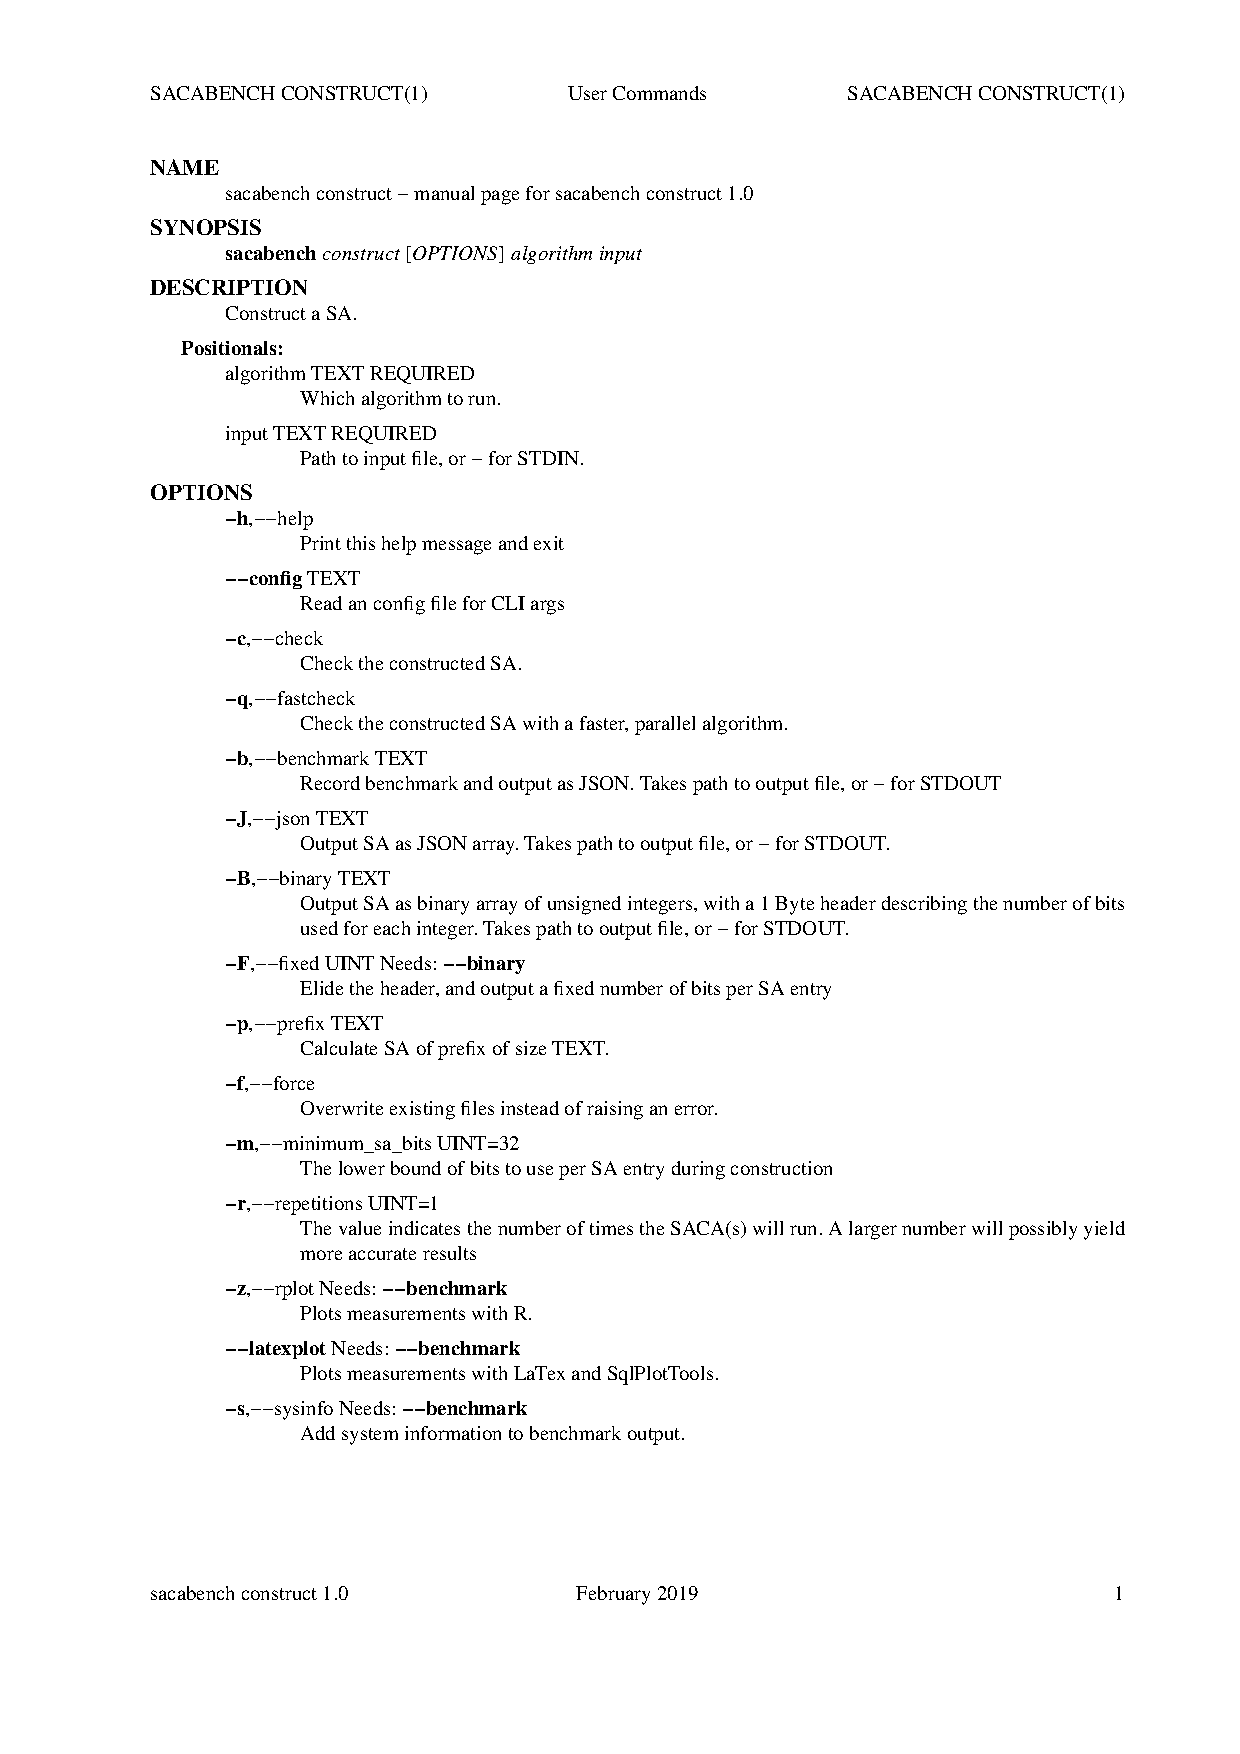
\includegraphics[page=1, viewport=0cm 32.8cm 20.5cm 68.5cm, clip, width=.5\textwidth]{{kapitel/3_framework/cli/sacabench-construct/sacabench-construct}.pdf}\\
    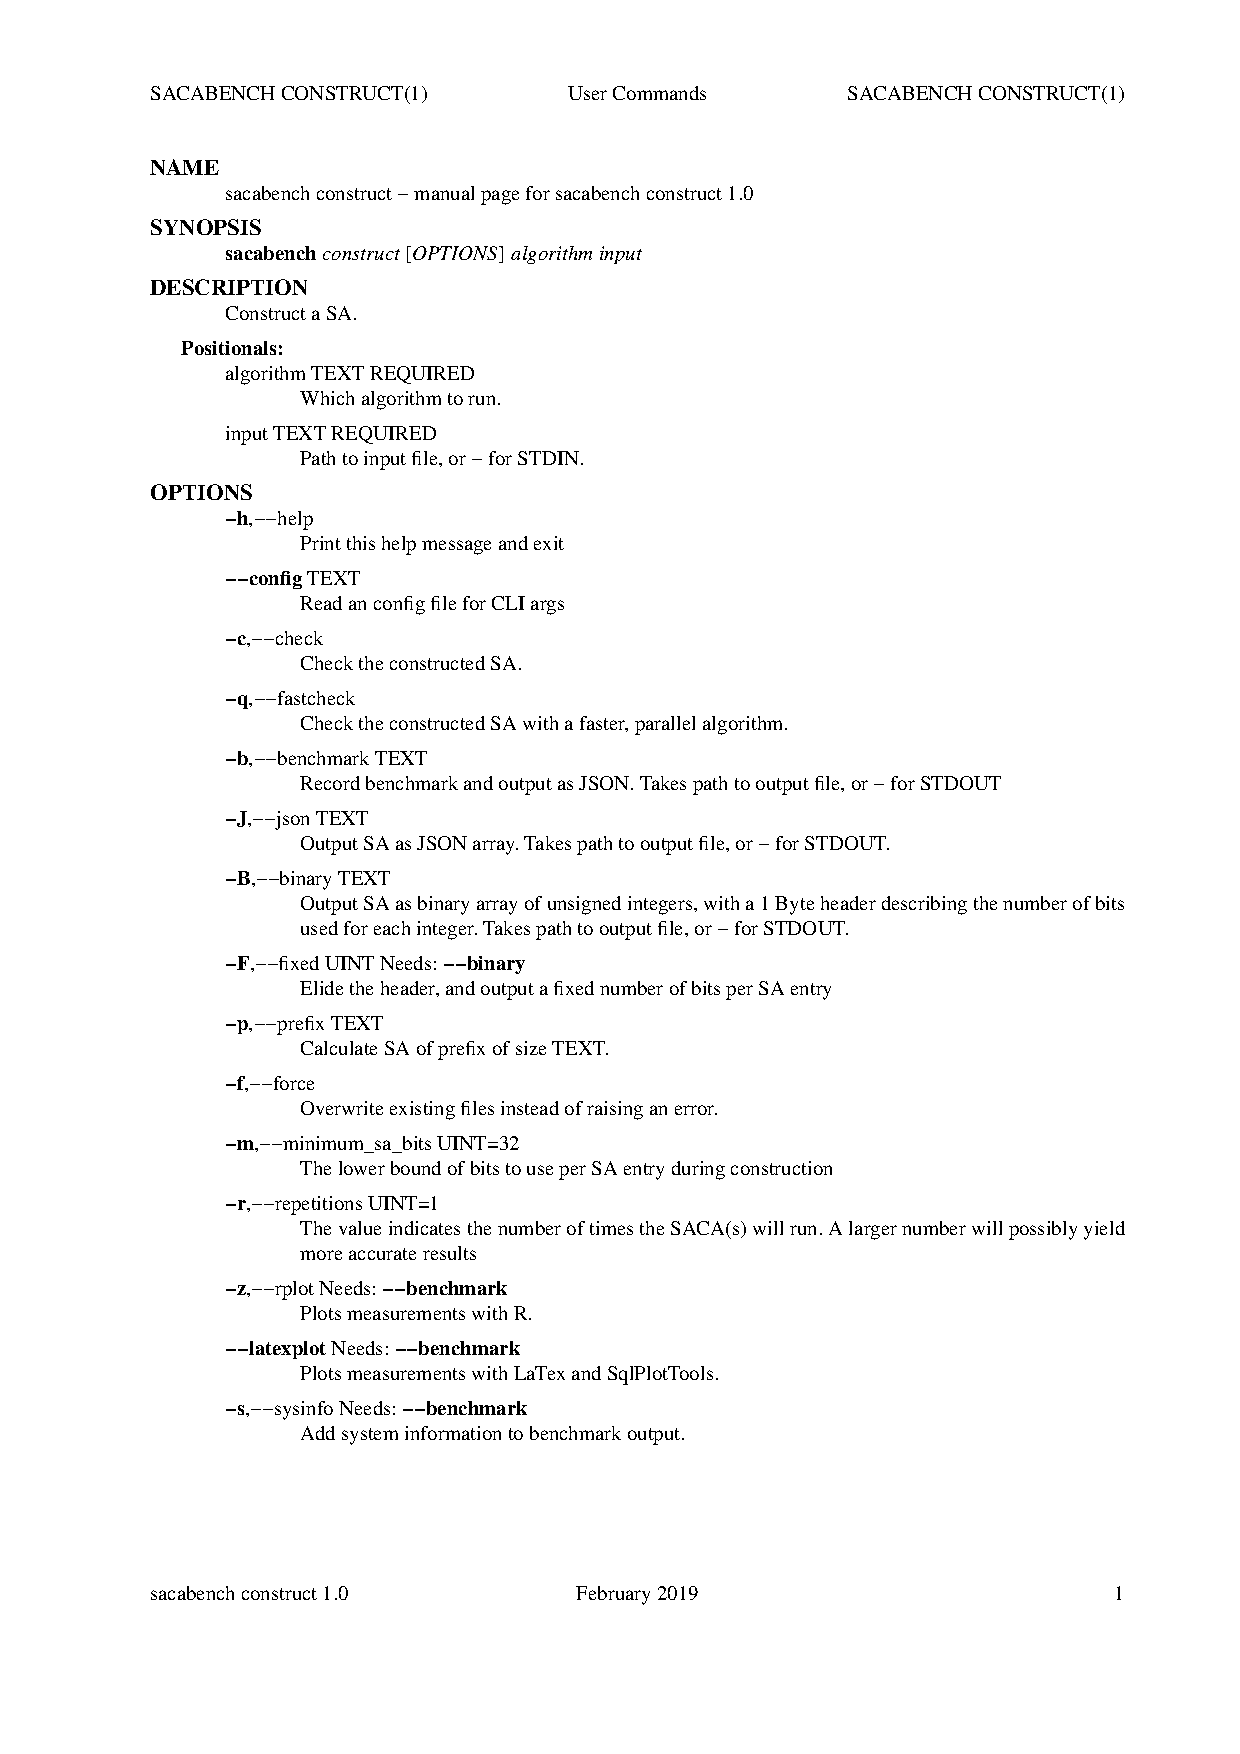
\includegraphics[page=1, viewport=0cm 25cm 20.5cm 26.3cm, clip, width=.5\textwidth]{{kapitel/3_framework/cli/sacabench-construct/sacabench-construct}.pdf}\\
    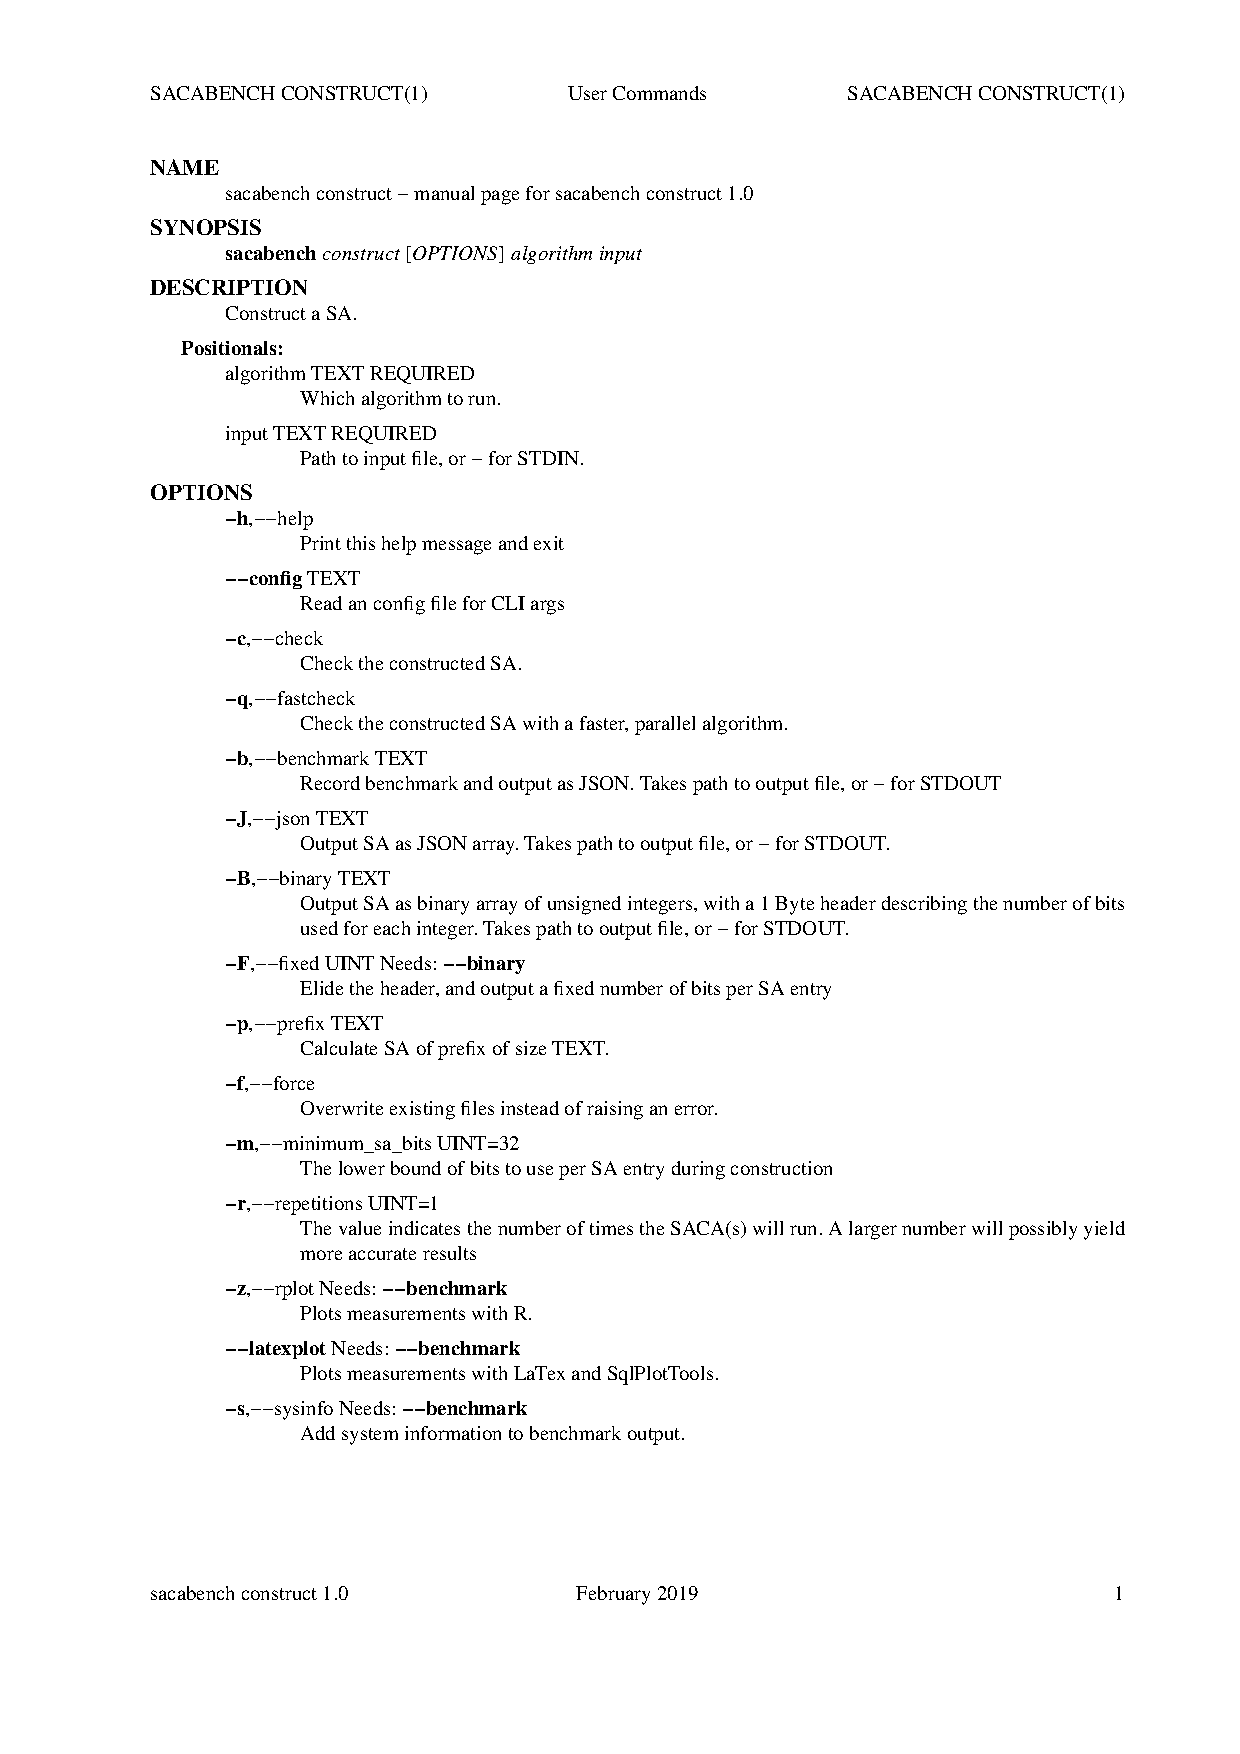
\includegraphics[page=1, viewport=0cm 0cm 20.5cm 1.5cm, clip, width=.5\textwidth]{{kapitel/3_framework/cli/sacabench-construct/sacabench-construct}.pdf}
    \caption{Gekürzte Ausgabe von \texttt{man sacabench construct}.}
    \label{manpage:sacabench-construct}
\end{wrapfigure}

Mit dem Befehl \texttt{sacabench construct} kann ein ausgewählter Algorithmus ausgeführt werden. 
\par
Der auszuführende Algorithmus wird dabei durch sein Kürzel bestimmt, wie es bei \termfont{sacabench list} angegeben ist. 
Gefolgt wird der Name des Algorithmus durch den Text, auf den er angewendet werden soll. 
Hierfür kann ein Pfad zu einer Textdatei oder alternativ \termfont{-} für STDIN angegeben werden. 
\par
Zusätzlich kann eine ganze Reihe von Optionen angegeben werden. 
Wie auch bei anderen Subcommands zeigen \termfont{-h} und \termfont{-{}-help} die Hilfe an. 
Die Option \termfont{-c} bzw. \termfont{-{}-check} wendet zusätzlich zu dem ausgewählten Algorithmus einen weiteren SACA auf die Eingabe an und überprüft, ob die beiden Ergebnisse gleich sind. 
Ist dies nicht der Fall, wird eine Fehlermeldung angezeigt. 
Eine Alternative hierzu ist die Option \termfont{-q} oder \termfont{-{}-quick}, welche auch die Korrektheit überprüft, jedoch einen parallelen Algorithmus verwendet. 
Wird die Option \termfont{-b} oder \termfont{-{}-benchmark} gefolgt von einem Pfad angegeben, wird an diesem Pfad eine JSON-Datei mit den gemessenen Zeiten und Speicherverbrauch angelegt. 
<<<<<<< HEAD
Existiert an dem angegebenen Pfad bereits eine Datei, kann diese mit der Option \termfont{-f} bzw. \termfont{-{}-force} überschrieben und durch die neue Messung ersetzt werden. 
Der Inhalt dieser Datei ist die Grundlage für die durch ein R-Skript erstellten Diagramme, welche mit \termfont{-z} oder \termfont{-{}-rplot} bei der Ausführung des Algorithmus generiert werden. 
Als Alternative hierzu können durch die Option \termfont{-{}-latexplot} auch Plots durch SqlPlotTools und Latex generiert werden.
Weitere Informationen hierzu sind in Kapitel \ref{framework:bechmark:sqlplottools} enthalten.
Um bei den Messungen ein besseres Ergebnis zu erhalten, kann mit der Option \termfont{-r} bzw. \termfont{-{}-repetitions} eine Anzahl an Durchführungen festgelegt werden. 
Hierdurch wird die Genauigkeit der Messung erhöht, indem das Arithmetische Mittel gebildet wird.
Weiterhin kann dem Befehl \termfont{-p} oder \termfont{-{}-prefix} hinzugefügt werden. 
Hierbei kann die Anzahl an führenden Bytes angegeben werden, die von der Eingabe verarbeitet werden sollen.
Um größere Werte leichter angeben zu können, sind die abkürzenden Schreibweisen K und M erlaubt, welche für Kilobyte bzw. Megabyte stehen.
Dies sorgt dafür, dass von der übergebenen Textdatei nur so viele Bytes verarbeitet werden, wie durch diese Option angegeben werden. 
Die Option \termfont{-B} oder \termfont{-{}-binary} veranlasst das Framework zur Ausgabe in binärer Form.
Anschließend werden die Einträge des Ergebnisses als Binärzahlen mit bis zu 8 Bits ausgegeben. 
Die erste Zahl der Ausgabe gibt die genaue Anzahl der Stellen an.
Ist eine feste Anzahl an Bits gewünscht, kann diese mit der Option \termfont{-F} bzw. \termfont{-{}-fixed} angegeben werden.
Alternativ kann das Framework das Suffixarray als JSON-Array ausgeben. 
Dies ist mit der Option \termfont{-J} oder \termfont{-{}-json} möglich.
Die nächste Option, welche dem Subcommand \texttt{sacabench construct} übergeben werden kann, ist \termfont{-m} oder \termfont{-{}-minimum\_sa\_bits} gefolgt von einem UINT Wert. 
Dieser Parameter bestimmt die Anzahl der Bits, die für die Datenstrukturen während der Berechnung genutzt werden.
Durch \termfont{-s} oder \termfont{-{}-sysinfo} werden Information über das System, welches das Benchmarktool ausführt, in die Ergebnisdatei mit aufgenommen.
Anstatt die genannten Optionen einzeln anzugeben, kann auch eine Konfigurationsdatei eingelesen werden, welche Werte für die zu benutzenden Optionen angibt.
Diese Datei ist im ini-Format und anstelle der Optionen wird die Option \termfont{-{}-config} gefolgt zu dem Pfad zu der Konfigurations-Datei beim Aufruf dieses Befehls angegeben.
Ein Beispiel für solch eine Konfigurations-Datei ist in Abbildung \ref{sacabench-construct:config} zu sehen.
Soll das Tool beispielsweise für den SACA \texttt{BPR} mit der angezeigten Konfigurationsdatei aufgerufen werden, sieht der entsprechende Befehl folgendermaßen aus:

\termfont{sacabench/sacabench construct --config /pfad/zur/config BPR \linebreak /pfad/zum/input/text}

Die gezeigte Konfigurations-Datei ist gleichbedeutentd zum Aufruf mit den Optionen \termfont{-c}, \termfont{-b}, \termfont{-f}, \termfont{-p 1K}, \termfont{-r 2}, \termfont{--rplot} und \termfont{--latexplot}.
Sollen die Optionen einzeln übergeben werden, ist dies mit diesem Aufruf möglich:

\termfont{sacabench/sacabench construct -c -b /ziel/pfad/zur/ergebnis.json -f -p 1K -r 2 --rplot --latexplot BPR /pfad/zum/input/text}
\par
}
\begin{figure}[!h]
\begin{minted}
[
frame=lines,
framesep=2mm,
baselinestretch=1.2,
fontsize=\footnotesize,
linenos,
numbersep=-4mm,
breaklines,
escapeinside=@@,
frame=single,
framesep=14pt
]
{text}
check = true
benchmark = /ziel/pfad/zur/ergebnis.json
force = true
prefix = 1K
repetitions = 2
rplot = true
latexplot = true
\end{minted}
\caption[Beispiel für eine Konfigurations-Datei für den Befehl \texttt{sacabench construct}]{Beispiel für eine Konfigurations-Datei für den Befehl \texttt{sacabench construct}}
\label{sacabench-construct:config}
\end{figure}
